\chapter{Industry Experience}
\label{chap:industryExperience}

\section{Introduction}
\label{sec:industryExperience-Introduction}

Business process mining, or process mining for short, aims at the automatic construction of models explaining the behavior observed in the event log[4]. For example, based on some event log, one can construct a process model expressed in terms of a Petri net. 

Over the last couple of years many tools and techniques for process mining have been developed [1][2][3]. Although process mining is very promising, most of the techniques make assumptions which do not hold in practical situations. For example, some techniques assume that there is no noise and have difficulties dealing with exceptions. Other approaches are limited to processes having a particular structure. Therefore, it is important to confront existing tools and techniques with event logs taken from real-life applications.

In this paper, the business discovery has been experienced using different existing process mining tools(ProM6, Apromore,Fluxicon Disco) .

\section{Methodology}
\label{sec:industryExperience-Methodology}

\subsection{Data}
The data come from a Saas ERP system called NetSuite, there is a functionality called save search, which is similar with SQL query to extract data from NetSuite live database~\ref{figure:saveSearch}

\begin{figure}[!htb]
    \centering 
    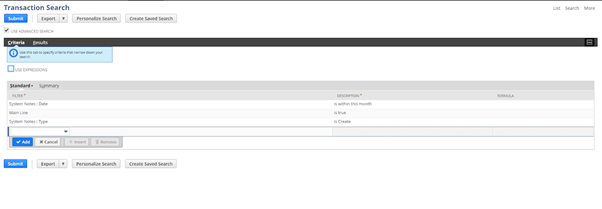
\includegraphics[scale=0.7]{resource/data.png}
    \caption{extracting data interface}
    \label{figure:saveSearch}
\end{figure}

DESCRIBE THE SQL QUERY.

\subsection{Data cleaning}

\section{Process mining tools}
\subsection{ProM}
ProM is an extensible framework that supports a wide variety of process mining techniques in the form of plugins. 
It is platform independent as it is implemented in Java, and can be downloaded free of charge. It provides different import data formats, like XES, XML, JSON.
\subsection{Apromore}
Apromore is an open-source process model repository. Its source code is available under the GNU Lesser General Public License.Apromore’s basic features include model import and export, version control and modeling support for a variety of languages, e.g., BPMN,
eEPC, YAWL, and Petri nets. It also supports CSV import. However, they required a format for CSV files 

\section{Use of listings}

Listings is a package to describe source code.

